\subsection{Deadlock}

\subsubsection*{Code}

\inputgroovy[label=Client.groovy]{../ChapterExamples/src/c07/Client.groovy}

\inputgroovy[label=RunDeadlockedCrossedClients.groovy]{../ChapterExamples/src/c07/RunDeadlockedCrossedClients.groovy}

\inputgroovy[label=Server.groovy]{../ChapterExamples/src/c07/Server.groovy}

\subsubsection*{Results}

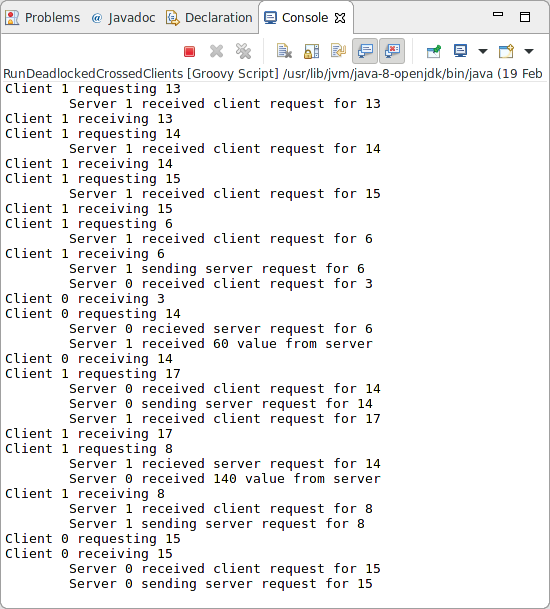
\includegraphics[width=\textwidth]{img/screenshots/7-1.png}

We can see from the results that the program deadlocks when both servers send a request to the other for information.  This causes both servers to lock on line 39 \mintinline{groovy}{thisServerRequest.write(key)}.  As they are both attempting to write to the other, neither can read and break the deadlock.